% -*- coding: utf-8 -*-
\chapter{グラフ探索のためのデータ構造}
\label{ch:search-performance}

ヒューリスティック探索の効率は探索効率、つまり展開したノードの数によって測られる場合が多い。本書の多くの節は探索効率を上げるためのアルゴリズムについて解説している。
しかしヒューリスティック探索の実行時間とメモリ量はデータ構造の実装にも大きく左右される。

ヒューリスティック探索ではオープンリストとクローズドリストの2つのデータ構造を保持する。
オープンリストに必要なインターフェイスは必要な操作はエンキュー (enqueue, pop)とデキュー (dequeue, push)である。
クローズドリストに必要なインターフェイスは挿入 (insert)と重複検知のための検索 (find, lookup)である。

これらのデータ構造をどのように実装するかは探索の効率に大きな影響を与える。
歴史的な経緯からオープン・クローズドリストと呼ばれているが、リストとして実装するのは非効率的である。

これらを実装するための効率的なデータ構造はアルゴリズムと問題ドメインに依存する。
この章ではどのようなシチュエーションでどのようなデータ構造を使われるかを説明する。
この章は実践的に非常に重要な章である。
残念ながらヒューリスティック探索の研究論文のほとんどはこの章で扱われる内容について自明のものとして扱わない。あるいはこれらの内容を「コードの最適化」として論文中には明示しない。が、その実自明ではないので初学者の多くはここで苦労することになる。
データ構造について議論を行っている論文としては\cite{burns2012implementing}がある。

%まず、$f$値の定義域が連続値か離散値かは重要である。
%また、$f$値が単調増加するかどうか。これはヒューリスティックが無矛盾かどうかにも依存する。



\section{オープンリスト (Open List)}
\label{sec:open-list}
%\captionlistentry[todo]{openlist}
オープンリストのプライオリティキューの実装方法は様々ある。
$f$値が連続値 (e.g. 実数)である場合はヒープを使うことが多い。
$f$値の取りうる値が有限個であり、$f$値が同じノードが沢山ある場合はバケットで実装することが出来る。
また、そのような場合は$f$値が同じノードのうちどのノードを選ぶかの\define{タイブレーキング}{tiebreaking}{タイブレーキング}も重要になってくる。


\subsection{データ構造の選択}
\label{sec:priority-queue}

オープンリストは探索の中で沢山エンキューとデキューを行うため、これらの操作の計算時間が速いものを選択したい。
オープンリストのシンプルな実装方法としては二分ヒープがあげられる。二分ヒープはほとんどの言語の標準ライブラリにあるため実装が簡単である。
探索アルゴリズムはノードの数が膨大になることが多い。
計算量のオーダーで見ると単純な二分ヒープよりも\define{フィボナッチヒープ}{Fibonacci heap}{フィボナッチヒープ}が効率が良いが、定数項が大きいため多くの場合二分ヒープが採用される。
二分ヒープよりも効率が良いデータ構造として\define{基数ヒープ}{radix heap}{きすうヒープ}がある \cite{ahuja1990faster}。基数ヒープはエンキューできる数値は最後に取り出した数値以上のものであるという制約がある。A*探索はヒューリスティックが単調である場合この制約を満たす。
これらのヒープの実装や性質についてはIntroduction to Algorithmsを参照されたい \cite{cormen01}。

プライオリティ値が取る値が有限個である場合はバケットで実装をすることが出来る \cite{burns2012implementing}。プライオリティ値が取る値が$C_{min} \leq i \leq C_{max}$の整数値であるとする。
バケットは長さ$C_{max} - C_{min} + 1$の配列からなる。プライオリティ値が$i$の要素は配列の$i - C_{min}$番目の位置にあるリストに追加される。バケットはエンキューもデキューも$O(C_{max} - C_{min})$で計算でき、保持しているノードの数に依存しない。そのため二分ヒープよりも高速であることが多い。
後述するタイブレーキングを行う場合はバケットの中に更に二段階目のバケットを用意することもできる \cite{burns2012implementing}。

\begin{figure}
  \centering
  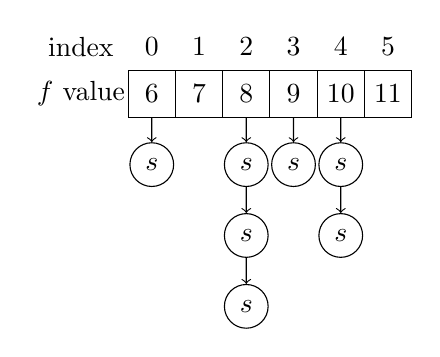
\begin{tikzpicture}[scale=0.6]
    % Array
\draw (0, 0) grid (6, 1);

% f-value and index
\foreach \x in {0, 1, ..., 5} {
  \pgfmathsetmacro{\fval}{int(\x + 6)}
  \node (f\x) at (\x + 0.5, 0.5) {\fval};
  \node (i\x) at (\x + 0.5, 1.5) {\x};
}

% label
\node (f) at (-1, 0.5) {$f$ value};
\node (i) at (-1, 1.5) {index};


% items
\node at (0 + 0.5, -1) [circle, draw] (n01) {$s$};
\draw[->] (0 + 0.5, 0) -- (n01);

\node at (2 + 0.5, -1) [circle, draw] (n21) {$s$};
\node at (2 + 0.5, -2.5) [circle, draw] (n22) {$s$};
\node at (2 + 0.5, -4) [circle, draw] (n23) {$s$};
\draw[->] (2 + 0.5, 0) -- (n21);
\draw[->] (n21) -- (n22);
\draw[->] (n22) -- (n23);

\node at (3 + 0.5, -1) [circle, draw] (n31) {$s$};
\draw[->] (3 + 0.5, 0) -- (n31);

\node at (4 + 0.5, -1) [circle, draw] (n41) {$s$};
\node at (4 + 0.5, -2.5) [circle, draw] (n42) {$s$};
\draw[->] (4 + 0.5, 0) -- (n41);
\draw[->] (n41) -- (n42);


  \end{tikzpicture}
  \caption{バケットによるオープンリストの実装 ($C_{min} = 6$, $C_{max} = 11$)}
  \label{fig:bucket}
\end{figure}


\subsection{タイブレーキング (Tiebreaking)}
\label{sec:tiebreaking}

\ref{ch:blind-search}章、\ref{ch:heuristic-search}章ではオープンリストでどのノードを最初に展開するかによってアルゴリズムの性能が大きく変わることを示してきた。
例えばA*探索では$f$値が最小のノードを優先して展開する (アルゴリズム\ref{alg:astar-search})。
だが、$f$値が最小のノードは複数ある場合がある。コスト関数が離散値である場合は$f$値が同じノードが大量にあることが多い。
このような場合、同じ$f$値のノードの中からどのノードを選ぶかを決定することを\define{タイブレーキング}{tie-breaking}{タイブレーキング}と呼ぶ。

A*探索で広く使われるタイブレーキング戦略は$h$値が小さいノードを優先させる方法である。$\arg \min_{u' \in Open} f(u')$を選択する代わりに以下の条件を満たす$u$を選択する。

\begin{align*}
  u =& \arg \min_{v \in B} h(v) \\
  s.t. \; \; & B = \{v | v \in Open, f(v) = \min_{v' \in Open} f(v')\}
\end{align*}

$h$値が小さいノードを優先させる理由としては、$h$値がゴールへの距離の推定だからである。なのでゴールに近いノードから展開したほうがゴールにたどり着くのが早いはずだ、というヒューリスティックである。

もう一つはLast-in-first-out (LIFO)タイブレーキングがよく使われる。
LIFOは最後にオープンリストに入ったノードから優先して展開する。
LIFOを使うメリットはオープンリストをバケット実装している場合に配列の一番後ろのノードがLIFOで得られるノードであることである。
\ref{sec:priority-queue}節にあるようにバケットは配列で実装されることが多いが、配列の末尾のノードを取り出すには定数時間しかかからない。なので自然にバケットを実装するとLIFOになる。

%逆にFirst-in-first-out (FIFO)にすると

タイブレーキングは長い間ヒューリスティック探索研究の中であまり重要視されておらず、よいヒューリスティック関数をデザインすることと比較してアルゴリズムの効率に対してあまり影響を及ぼさないと考えられてきた。
近年の研究でタイブレーキングが重要なファクターになる場合があるということが実験的に示された \cite{asai2016tiebreaking}。


\section{クローズドリスト (Closed List)}
\label{sec:closed-list}

重複検出は無駄な展開を防ぐために不可欠な操作である。
非明示的状態空間グラフではあらかじめすべての状態を知ることが出来ないので、探索中に発見された状態の集合を保持しておくための動的な辞書が必要になる。

クローズドリストは生成済み・展開済みノードを保持し、新しくノードが生成されたときにすでにその中にあるかどうかを確かめる。
一般的に辞書のデータ構造は挿入 (insert)、検索 (lookup)、削除 (delete)をサポートするが、探索アルゴリズムに必要なのは挿入と検索である。

クローズドリストの実装には\define{ハッシュテーブル}{hash table}{ハッシュテーブル}が用いられることが多い。
ハッシュテーブルは探索で一番頻繁に使われる検索が定数時間で出来るためである。


\subsection{ハッシュテーブル (Hash Table)}
\label{sec:hash-table}

集合$U = \{0, 1, ..., N - 1\}$をキーの候補とする\define{辞書}{dictionary}{じしょ}は、保持されたキーの集合$R \subseteq U$から連想情報の集合$I$への部分写像である。
グラフ探索において状態$s \in S$を一意に表すためのキーを$k(s)$とする ($k: S \rightarrow U$)。
キーは更にハッシュテーブルと呼ばれる配列$T[0, ..., m-1]$に写される。この写像$h: U \rightarrow \{0, ..., m-1\}$を\define{ハッシュ関数}{hash function}{ハッシュかんすう}と呼ぶ。簡単のためここでは状態から配列のインデックスまでの関数$S \rightarrow \{0, ..., m-1\}$を$h$を使って表す。

多くの場合$N > m$なので、このハッシュ関数は単射ではない。よって異なるキーがハッシュテーブル上の同じ位置に配置されることになる。これをハッシュの\define{衝突}{hash collision}{しょうとつ}と呼ぶ。
ハッシュテーブルへのアクセスにかかる時間は1. ハッシュ値の計算、2. 衝突時の処理方法、3. 保持されたキーの数とハッシュテーブルの大きさの比に依存する。

ハッシュ関数の選択はハッシュテーブルの性能に大きく影響を与える。最悪の場合、すべてのキーがテーブルの同じ位置に移される。最良の場合、一度も衝突が起こらず、アクセス時間は定数になる。最悪の場合の計算時間は理論的には興味のある話題だが、多くの場合正しくハッシュを計算することで避けられる。

衝突したハッシュの処理方法としては\define{連鎖法}{chaining}{れんさほう}と\define{開番地法}{open addressing}{かいばんちほう}がある。連鎖法はハッシュテーブルの各位置にリストが置かれ、その位置に挿入された連想情報はそのリストに順次追加されていく。同じ位置に$n$個の状態が挿入された場合リストの長さは$n$になる。このとき、ここの位置への検索の速度は$O(n)$となる。開番地法は衝突した場合テーブル中の空いている別の位置を探し、そちらに入れる方法である。探索アルゴリズムにおいては連鎖法が使われることが多い。


\subsection{ハッシュ関数 (Hash Function)}
\label{sec:hash-function}

{\bf 良い}ハッシュ関数に求められる要件は主に2つである。
一つはハッシュ値が値域内でなるべく均等に分散してほしい。
もう一つはハッシュの計算に時間がかからない方が良い。

グラフ探索のためのハッシュ関数をデザインするために考えなければならないのは、探索中に現れる状態集合、探索空間は状態空間全体のほんの一部であり、かつ偏りのある集合であるということである。
ハッシュ関数はその探索空間内でハッシュ値が十分に均等であってほしい。


\subsubsection{剰余法 (Remainder Method)}

$k(s)$を整数と考えることが出来るならば、それを$m$で割った余りをハッシュ値として使える。

\begin{equation}
  h(s) := k(s) \; \text{mod} \; m
\end{equation}
  
このハッシュ関数は$S$から$T$への写像になる ($h: S \rightarrow \{0, ..., m-1\}$)。$T$へ均等に分配するためには法$m$の選択が重要になる。
例えば$m$に2の倍数を選んでしまうと、$h(s)$が偶数であるのは$k(s)$が偶数であるときであり、そのときのみである (iff)。$m$が任意の数の倍数であると同様の不均一が起きてしまうので、$m$は素数を選ぶと良い。


\subsubsection{積算ハッシュ法 (Multiplicative Hashing)}
積算ハッシュ法はキー$k(s)$と無理数$\phi$の積の小数部分を使ったハッシュである。

\begin{equation}
	h(s) = \floor{m (k(s) \phi - \floor{k(s) \phi})}
\end{equation}

$\phi$はパラメータであり、$(\sqrt{5} - 1) / 2$の黄金比を使うと良いとされている。

\subsubsection{ハッシュの性質}

関連して、クローズドリストにとって良い性質のハッシュがいくつかある。

グラフ探索では状態遷移は状態の一部分のみに作用し、状態変数のほとんどは変わらないということが多い。このとき、新しい状態のハッシュ値を一から計算するのではなく、元の状態のハッシュ値と状態遷移による差分を利用して新しい状態のハッシュ値を求めることが出来る場合がある。この方法を\define{差分ハッシュ}{incremental hashing}{さぶんハッシュ}と呼ぶ。差分ハッシュはハッシュ値の計算時間を短くできることがある。

どのような操作があっても衝突が起こらないようなハッシュを\define{完全ハッシュ}{perfect hash function}{かんぜんハッシュ}と呼ぶ。もし$n = m$であれば最小完全ハッシュと呼ぶ。完全ハッシュがあればどのような操作も$O(1)$で行うことができる。
問題によって完全ハッシュは簡単に計算することが出来る。例えばスライディングタイルパズルであれば状態$s = (v_0, v_1,...,v_8)$に対して$h(s) = \sum_{i = 0..8} v_i \cdot 9^i$と単純に状態変数の列を使って計算することが出来る。ただし長さ$9^9$の配列は大きすぎるので工夫が必要になる。完全ハッシュを作るのは簡単だが、小さい完全ハッシュを作るのは難しい。スライディングタイルパズルは\define{辞書順}{lexicographical order}{じしょじゅん}によって最小完全ハッシュを作ることが出来る \cite{korf2005large}。


\subsection{トランスポジションテーブル (Transposition Table)}

木探索の問題点は重複検出を行わないため、同じ状態を複数回展開し、時間がかかってしまうことである。一方グラフ探索の問題点は重複検出を行うため、生成したノードの数だけメモリを消費することにある。
グラフが大きい場合はやがてメモリを使い果たし、探索が続けられなくなってしまう。
しかしながら、実はグラフ探索において重複検出は必ずしも正しくなければならないものではない。重複してノードを生成しても問題なくアルゴリズムは動作する。仮にクローズドリストの一部を捨ててもアルゴリズムの正しさを損なうものではない。

\define{トランスポジションテーブル}{transposition table}{トランスポジションテーブル}はこのアイディアに基づき、展開したノードの一部のみを保存することで重複検出をしつつメモリの消費を抑える手法である。
トランスポジションテーブルはグラフ探索におけるクローズドリストと同様、辞書である。
クローズドリストがすべての生成済みノードを保持していることを保証するのに対して、トランスポジションテーブルはそのような保証をしない。
トランスポジションテーブルはどのノードを保持し、どのノードを捨てるかを賢く選択しなければならない。どのノードを保持するべきかという戦略はいくつか提案されている \cite{breuker1994replacement,akagi2010transposition}。

単純なものとしては、テーブルが一杯になるまではすべてのノードをテーブルに追加し、テーブルが一杯になったらすべてのノードを捨てる戦略がある。
Stochastic node caching \cite{miura1999stochastic}は、新しく追加されたノードを確率$1-p$で捨てるというものである。この戦略だと$n$回訪れたノードは確率$1- (1-p)^n$でテーブルに追加されるため、たくさん訪れたノードほど重複検出されやすいことになるという点で合理的である。
2人ゲームでよく使われる戦略は、2つのノードのハッシュ値が衝突したらどちらか一方のみを残すという戦略である。より$d$値が大きい(深い)ノードを残す戦略が一般的である。この戦略はハッシュテーブルの衝突を減らせるという点で一挙両得になる。

トランスポジションテーブルはA*だけでなく後述するIDA* (節\ref{sec:depth-first-iterative-deepening})でも使われる \cite{reinefeld1994enhanced}。IDA*の空間量は最適解の深さに対して線形なので消費メモリが非常に少ない。あまったメモリを効率よく使うためにIDA*にトランスポジションテーブルを用いるという研究が多い \cite{reinefeld1994enhanced,akagi2010transposition,kishimoto:02}。

トランスポジションテーブルは元々2人ゲームの分野から発展した技術である。同じ手を異なる順番で行うことで同じ状態に到達することを検出するために使われていたのでtranspositionという名前になっている。


\subsection{遅延重複検出 (Delayed Duplicate Detection)}
\label{sec:delayed-duplicate-detection}

\ref{sec:graph-search-algorithm}節ではノードを生成したタイミングで重複検出を行うアルゴリズムを説明した。この方法だとノードが生成されたその瞬間に検出を行うという意味で\define{即時重複検出}{immediate duplicate detection}{そくじちょうふくけんしゅつ}と呼ぶことがある。
それに対して、ノードを展開するタイミングで検出を行う\define{遅延重複検出}{delayed duplicate detection}{ちえんちょうふくけんしゅつ}という方法もある \cite{korf2003delayed}。
ノードが生成された瞬間に重複検出を行わない場合、オープンリスト内に同じ状態を持ったノードが重複して存在する場合がある。
しかしノードを展開するときに重複検出を行うので、クローズドリストにノードの重複はない。
アルゴリズム\ref{alg:ddd}は遅延重複検出を用いる場合のグラフ探索アルゴリズムの疑似コードである。

遅延重複検出は展開ノード毎に重複検出の回数を減らすことができるというメリットがある。一方、オープンリスト内に重複が存在する可能性があるため、プライオリティの選択次第ではノードの再展開が増えてしまうデメリットがある。
そのため遅延重複検出はノードの重複が少ない問題や、重複検出に時間がかかる場合に使われる。特にクローズドリストをハードディスクなどの外部メモリに置く外部メモリ探索に相性が良い。


\begin{algorithm}
\caption{遅延重複検出を用いたグラフ探索}
\label{alg:ddd}
	\Input{非明示的状態空間グラフ $(s, Goal, Expand, w)$, プライオリティ関数 $f$}
	\Output{$s$からゴール状態$t \in T$への経路、経路が存在しなければ$\emptyset$}
	$Closed \leftarrow \emptyset$, $Open \leftarrow \{s\}$, $d(s) \leftarrow 0$, $g(s) \leftarrow 0$\;
	\While{$Open \neq \emptyset$} {
                $u \leftarrow \argmin_{u' \in Open} f(u')$ \;
	        $Open \leftarrow Open \setminus \{u\} $\;
          
		\If {$Goal(u)$} {
			\Return $Path(u)$\;
		}

                $s \leftarrow parent(u)$\;
		\If{$u \notin Closed$ {\bf or} $g(s) + w(s, u) < g(u)$} {
                  $d(u) \leftarrow d(s) + 1$\;
                  $d(u) \leftarrow g(s) + w(s, u)$\;
		  $parent(u) \leftarrow s$\;
		  \For {each $v \in Expand(u)$} {
		    $Open \leftarrow Open \cup \{v\}$\;
		    $parent(v) \leftarrow u$\;
		  }
		}

                \If{$u \notin Closed$} {
                  $Closed \leftarrow Closed \cup \{u\}$\;
                }
 	}
	\Return $\emptyset$\;
\end{algorithm}


% \subsection{関連文献}
% 
% \TODO{Rabin and Karp hashing}
% 
% \TODO{Universal hash function}


